\documentclass[12pt]{article}

% Language setting
% Replace `english' with e.g. `spanish' to change the document language
\usepackage[english]{babel}

% Set page size and margins
% Replace `letterpaper' with `a4paper' for UK/EU standard size
\usepackage[letterpaper,top=2cm,bottom=2cm,left=3cm,right=3cm,marginparwidth=1.75cm]{geometry}

\setlength{\parskip}{\baselineskip}%
\setlength{\parindent}{6pt}%https://www.overleaf.com/project/60d099109e0a9e26ca6f8f7d

% basic packages
\usepackage{setspace} % spacing

\setlength{\parindent}{2em}
\setlength{\parskip}{1em}

% Useful packages
\usepackage{amsmath}
\usepackage{subcaption}
\usepackage{graphicx}
\usepackage{booktabs}
\usepackage[colorlinks=true, allcolors=blue]{hyperref}
\usepackage[
backend = biber, 
style=apa, 
sorting=nty
]{biblatex}

\addbibresource{bibliography.bib} 

\title{Prelimitary Analysis of the Relationship Between Conlifct Measures and Nightlights in Thailand: Pre-Doc Evaluation Task for Wyss Academy at the University of Bern}
\author{Ying Yan}

\begin{document}
\maketitle

\section*{Introduction \& Background}

\textbf{Research Question:} Is there a relationship between conflict measure and nightlights in Thailand? How did this relationship change during the decade 2010-2020?

To answer this research question, two types of data are required: the conflict data and the nightlight data. Conflict data can be obtained from \textcite{davies_organized_2025}'s UCDP Georeferenced Event Dataset (GED), which contains disaggregated conflict data on conflict events for specific times and locations. To ensure data completeness, we will not select based on event location precision and conflict type at this stage. However, further arguments and concerns may be necessary in a later analysis.

Nightlights data is widely publicly available \footnote{e.g., \href{https://worldbank.github.io/OpenNightLights/wb-light-every-night-readme.html}{World Bank Light Every Night Data}, \textcite{Li2020}}. The two main sources of night lights data are the Defense Meteorological Satellite Program Operational Linescan System (DMSP), available until 2013, and the Day-Night Band (DNB) of the VIIRS onboard the Suomi satellite launched by NASA and the National Oceanic and Atmospheric Administration (NOAA) in 2011. The VIIRS data is more advanced, contains fewer errors, and is more suitable for research. To adjust for inconsistencies between the two datasets, \textcite{Li2020} integrated DMSP data with VIIRS data, making the night-light raster data consistent from 1992 to 2020. As the research question focuses on the recent decade, which includes a transition period in nightlight data technology and methodology, we use \textcite{Li2020} adjusted nightlight data for time-series comparison and analysis. It is also worth noting that \textcite{gibson_night_2020} discuss the potential risks of applying such data to economic analysis based on their underlying data collection methodology.

\newpage
\section{Asian Map}
Figure \ref{fig:asianmap} shows conflict measures and night-lights for countries in Asia, where Figure \ref{fig:asian2020} shows the measures for the year 2020 and Figure \ref{fig:asian2010} shows the measures for the year 2010. The maps on the left show only nightlights, while the maps on the right show conflict events (red dots) in each country, overlaid on the nightlights data.

\begin{figure}[!b]
     \centering
     \begin{subfigure}[b]{0.9\textwidth}
         \centering
         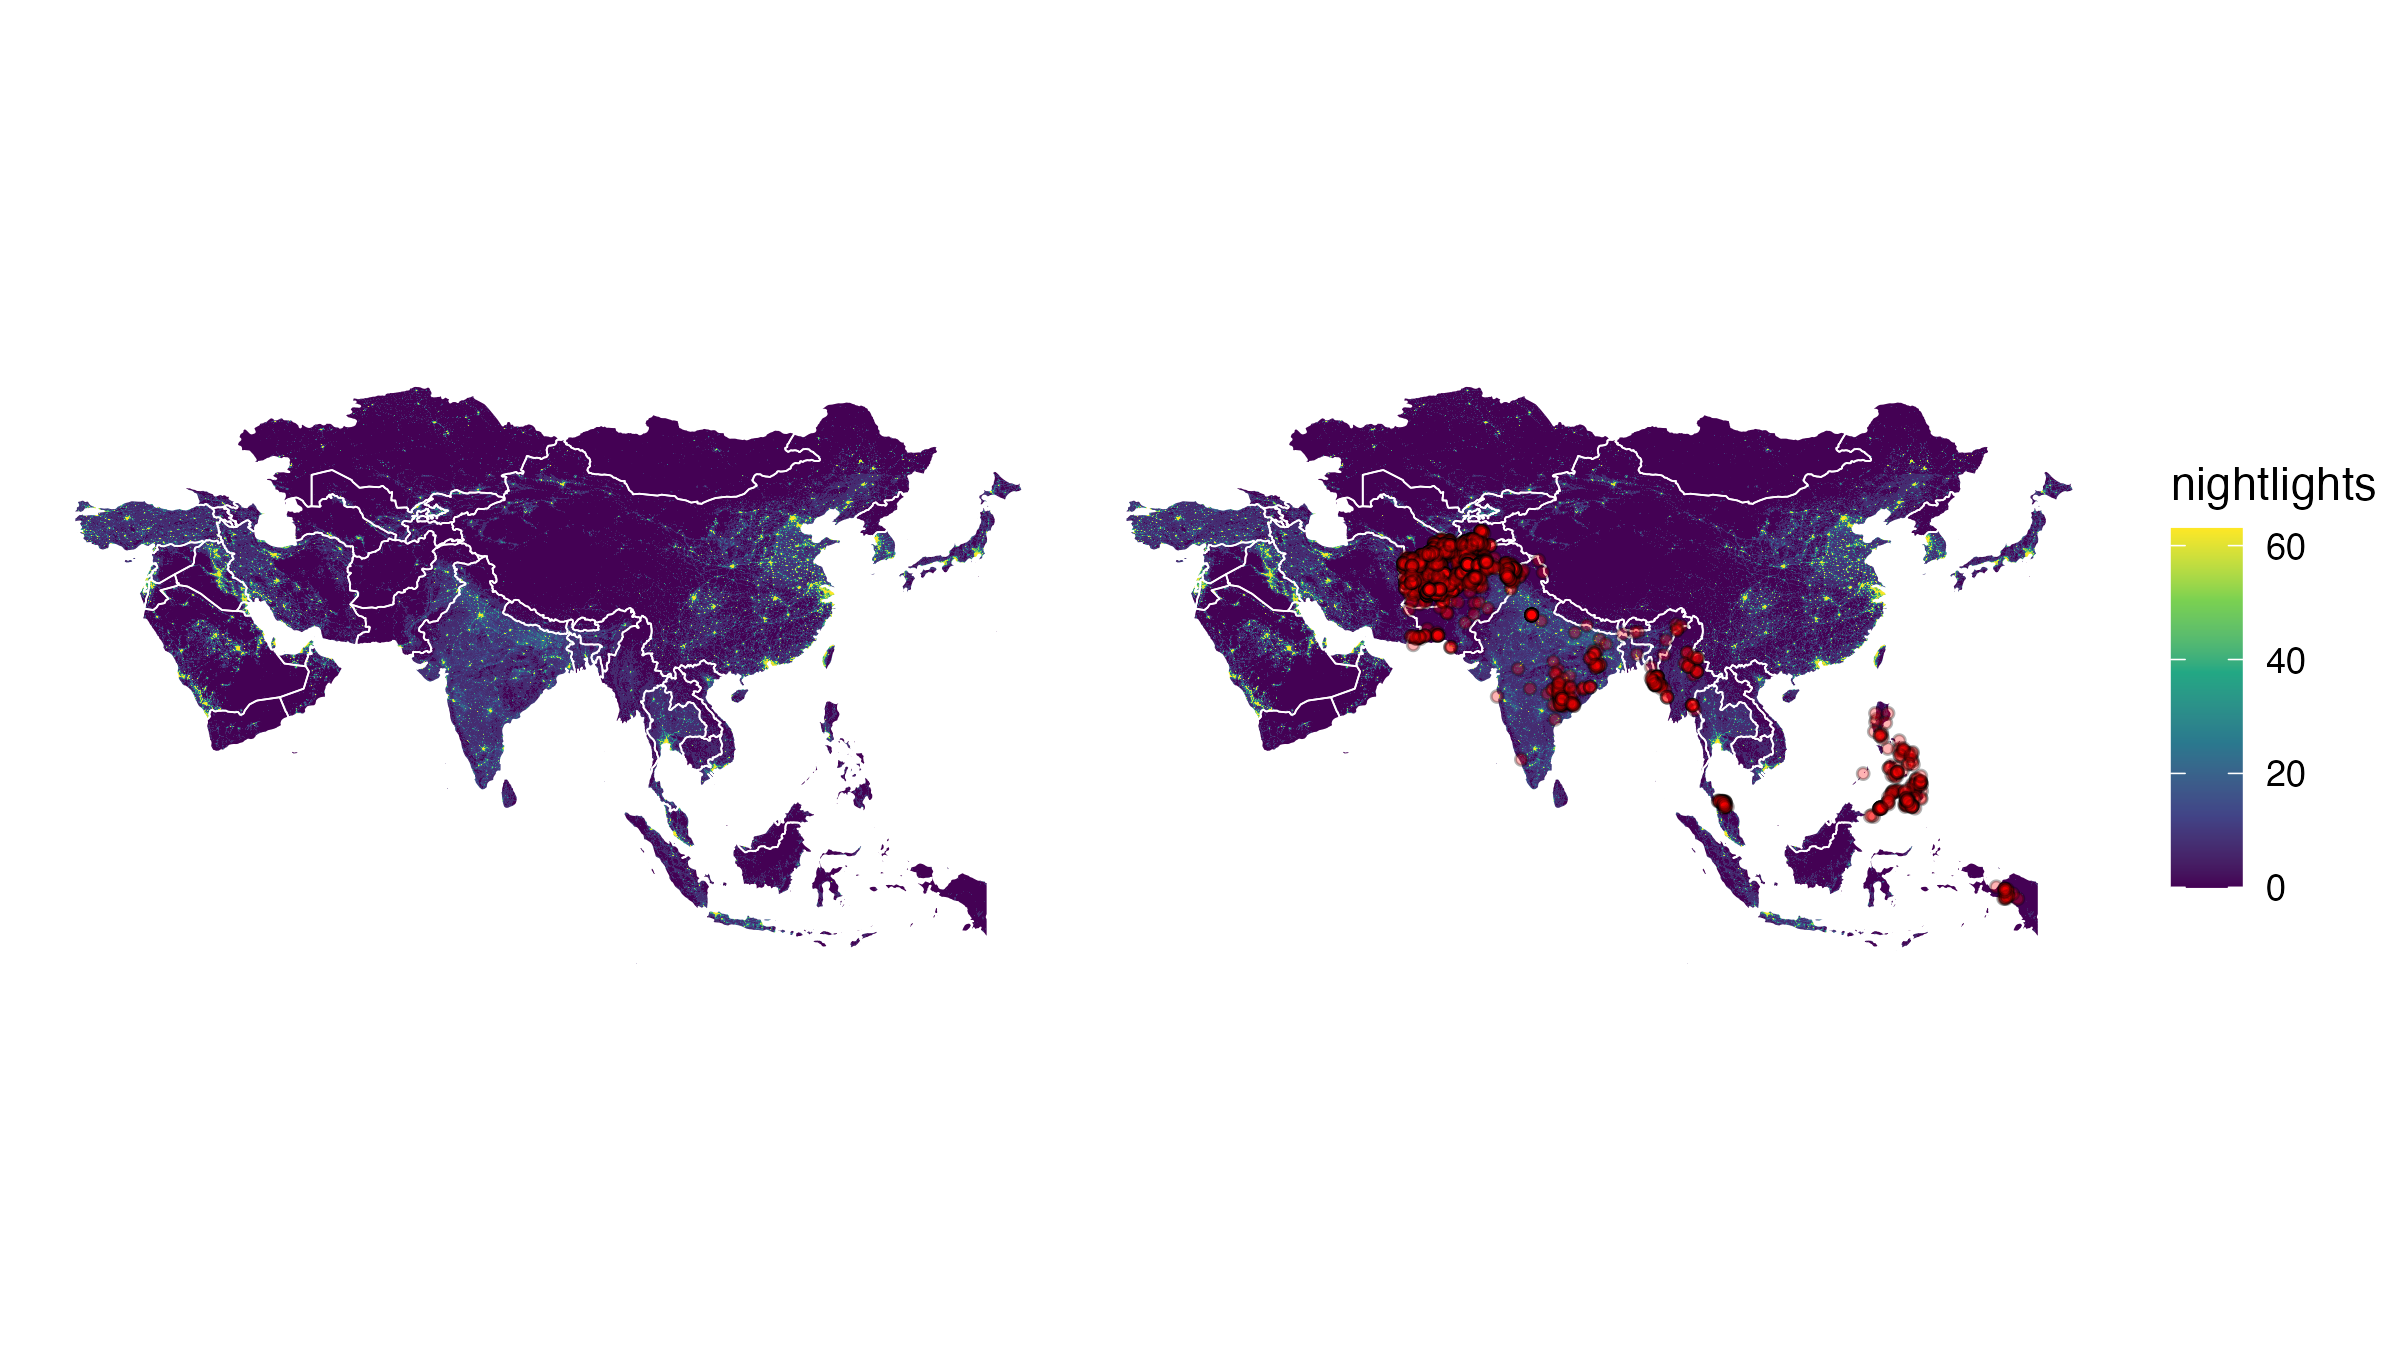
\includegraphics[width=\textwidth]{map_asian_2020.png}
         \caption{2020}
         \label{fig:asian2020}
     \end{subfigure}
     %\vskip\baselineskip
    \begin{subfigure}[b]{0.9\textwidth}
         \centering
         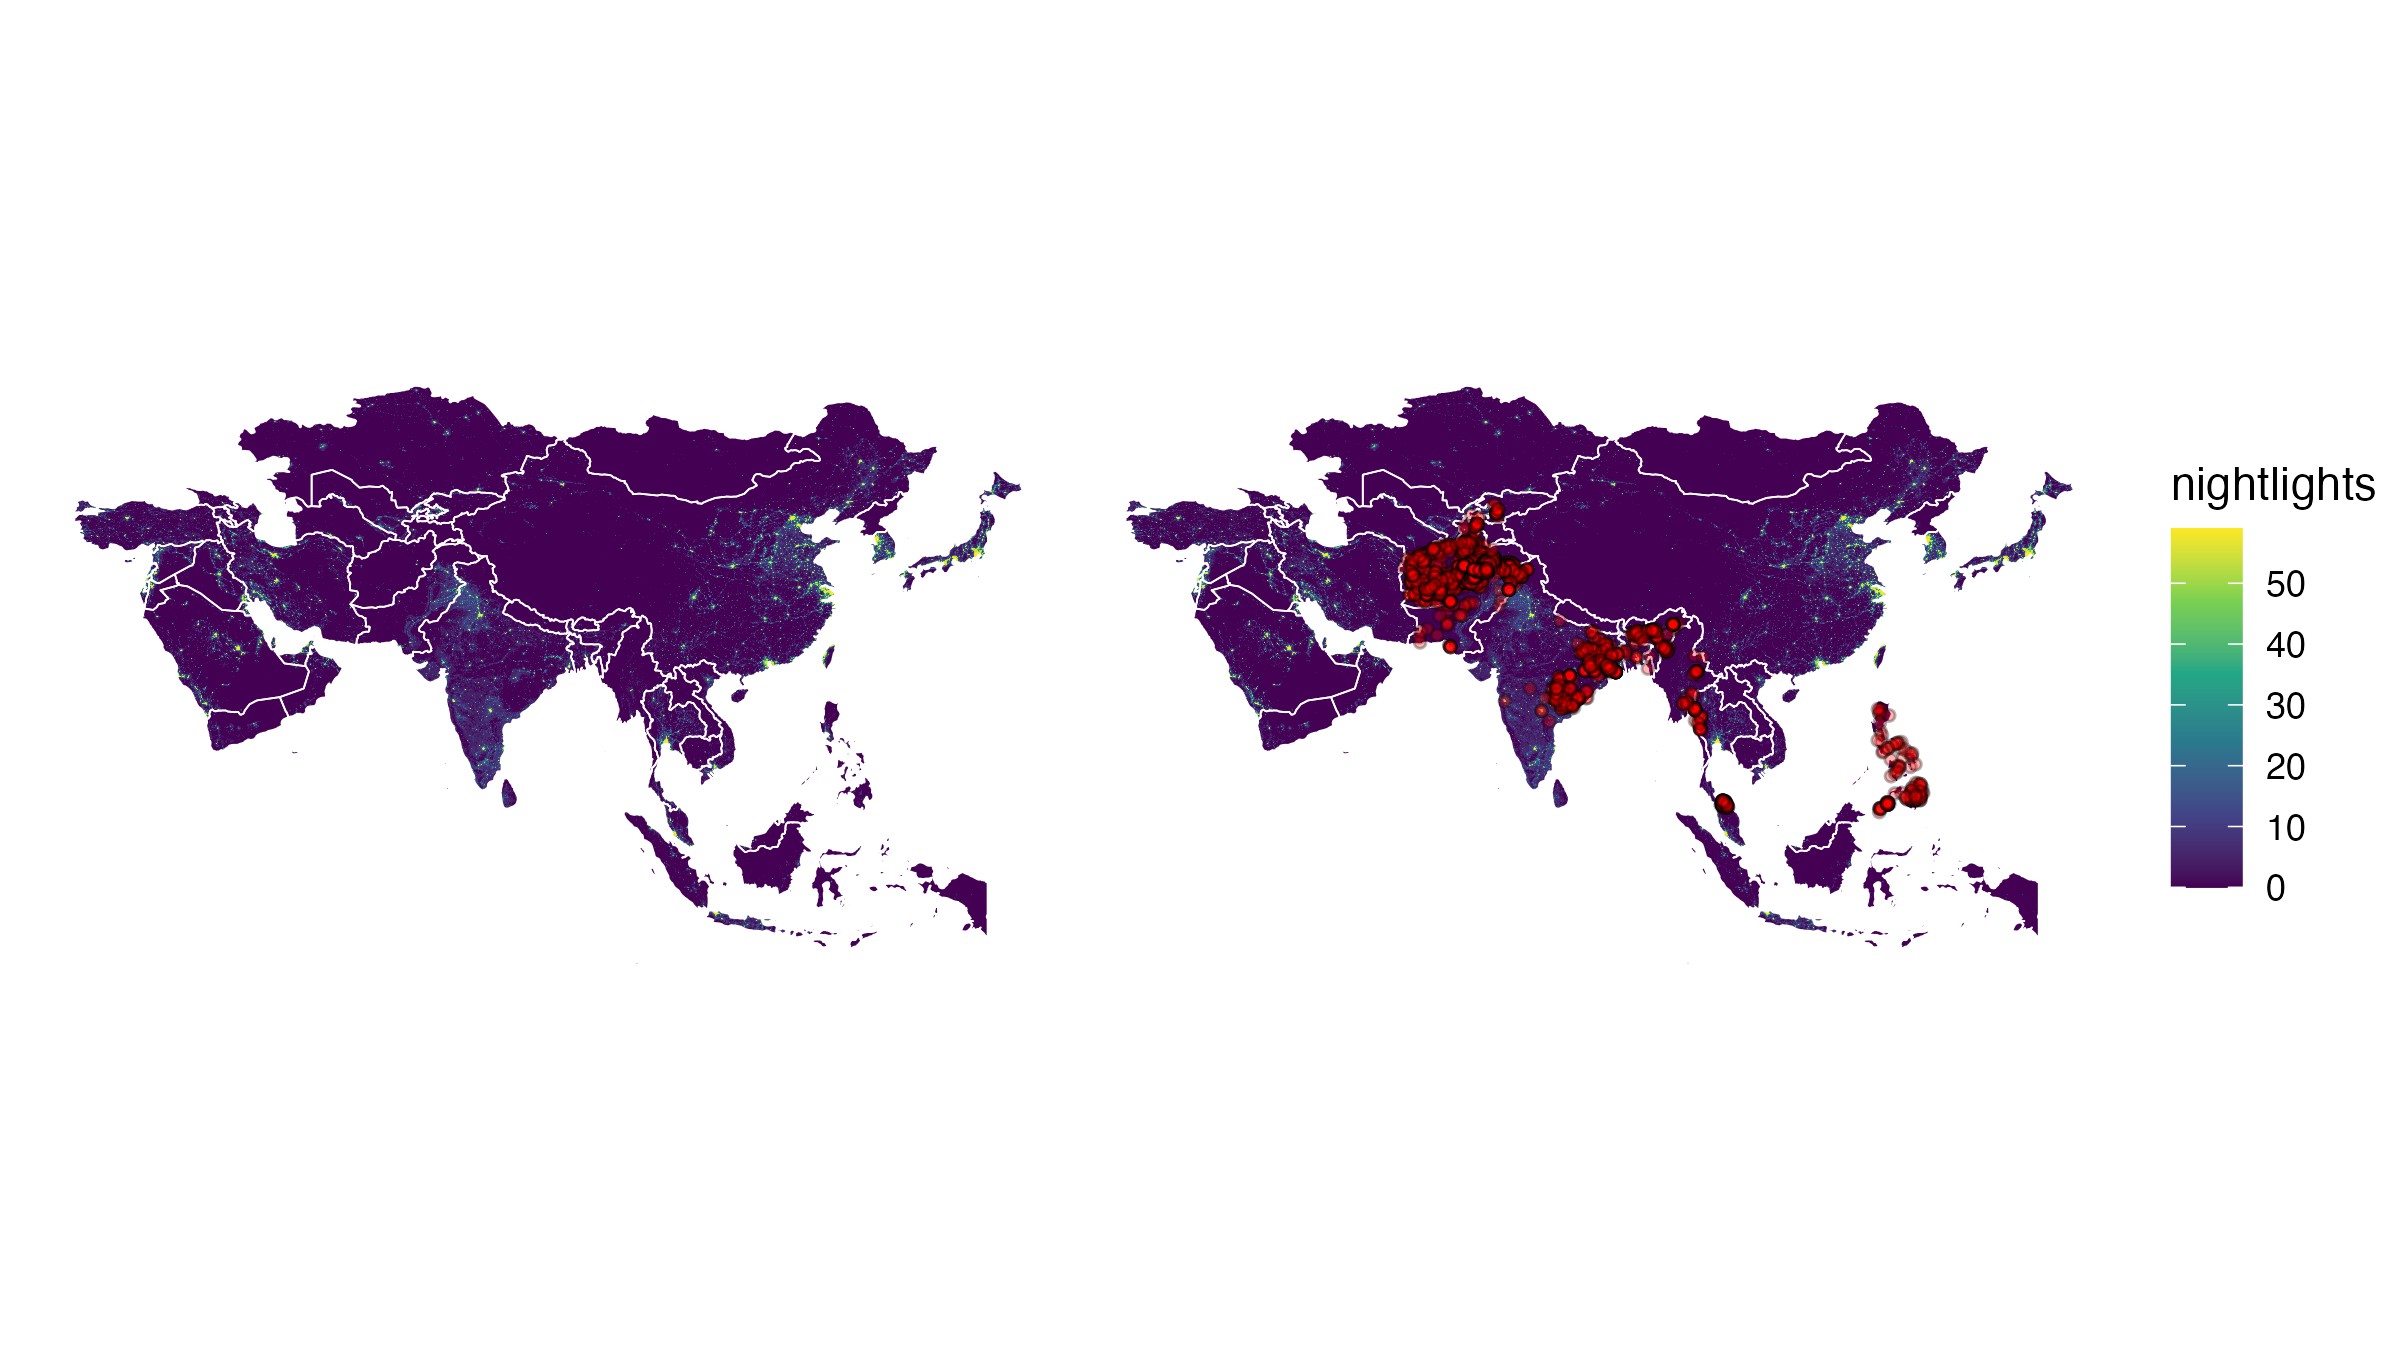
\includegraphics[width=\textwidth]{map_asian_2010.png}
         \caption{2010}
         \label{fig:asian2010}
    \end{subfigure}
    \caption{Conflict Events and Nightlight Intensity in Asia. Year 2020 vs 2010.}
    \label{fig:asianmap}
\end{figure}

The countries that have suffered the most from conflicts in Asia over the past decade are Afghanistan, India, Pakistan, the Philippines and Myanmar. Thailand is sixth (see the complete figures in the Appendix). By comparing areas of conflict with night-light intensity, a negative correlation between night-light usage and the concentration of conflict events can be identified. This negative correlation has also been consistent over time: for example, in 2010, night-light intensity was lower and conflict intensity was higher than in 2020.

\section{Thailand Map}
The comparison maps specifically of Thailand for year 2010 and 2020 are illustrated in Figure \ref{fig:thailandmap}, where Figure \ref{fig:thailand2020} shows the nightlights and conflict events happened in Thailand in 2020 and Figure \ref{fig:thailand2010} shows similar data in 2010. The red dots on the right of each figure indicate the number of conflicts that have been undergone in that year. The white lines on the map are the province borders, which are obtained from \href{https://gadm.org/download_country.html#google_vignette}{GADM}. 

The night-time light usage is concentrated around the capital, Bangkok, which is the area with the most active economic activities. The conflicts are concentrated in the southern provinces, due to the ongoing ethnic and religious separatist insurgencies in the three southernmost provinces (Southern border provinces) of Thailand, Pattani, Yala and Narathiwat from 2004 to the present (\cite{Payo01102024}). The insurgencies become more violent in early 2000s. 

The map indicates similar correlations between conflict events and nightlights as in Figure \ref{fig:asianmap} - conflicts are concentrated in areas with low night-time light usage, and in 2010, there were fewer night-time lights and more conflicts than in 2020.

\begin{figure}[ht]
     \centering
     \begin{subfigure}[b]{0.45\textwidth}
         \centering
         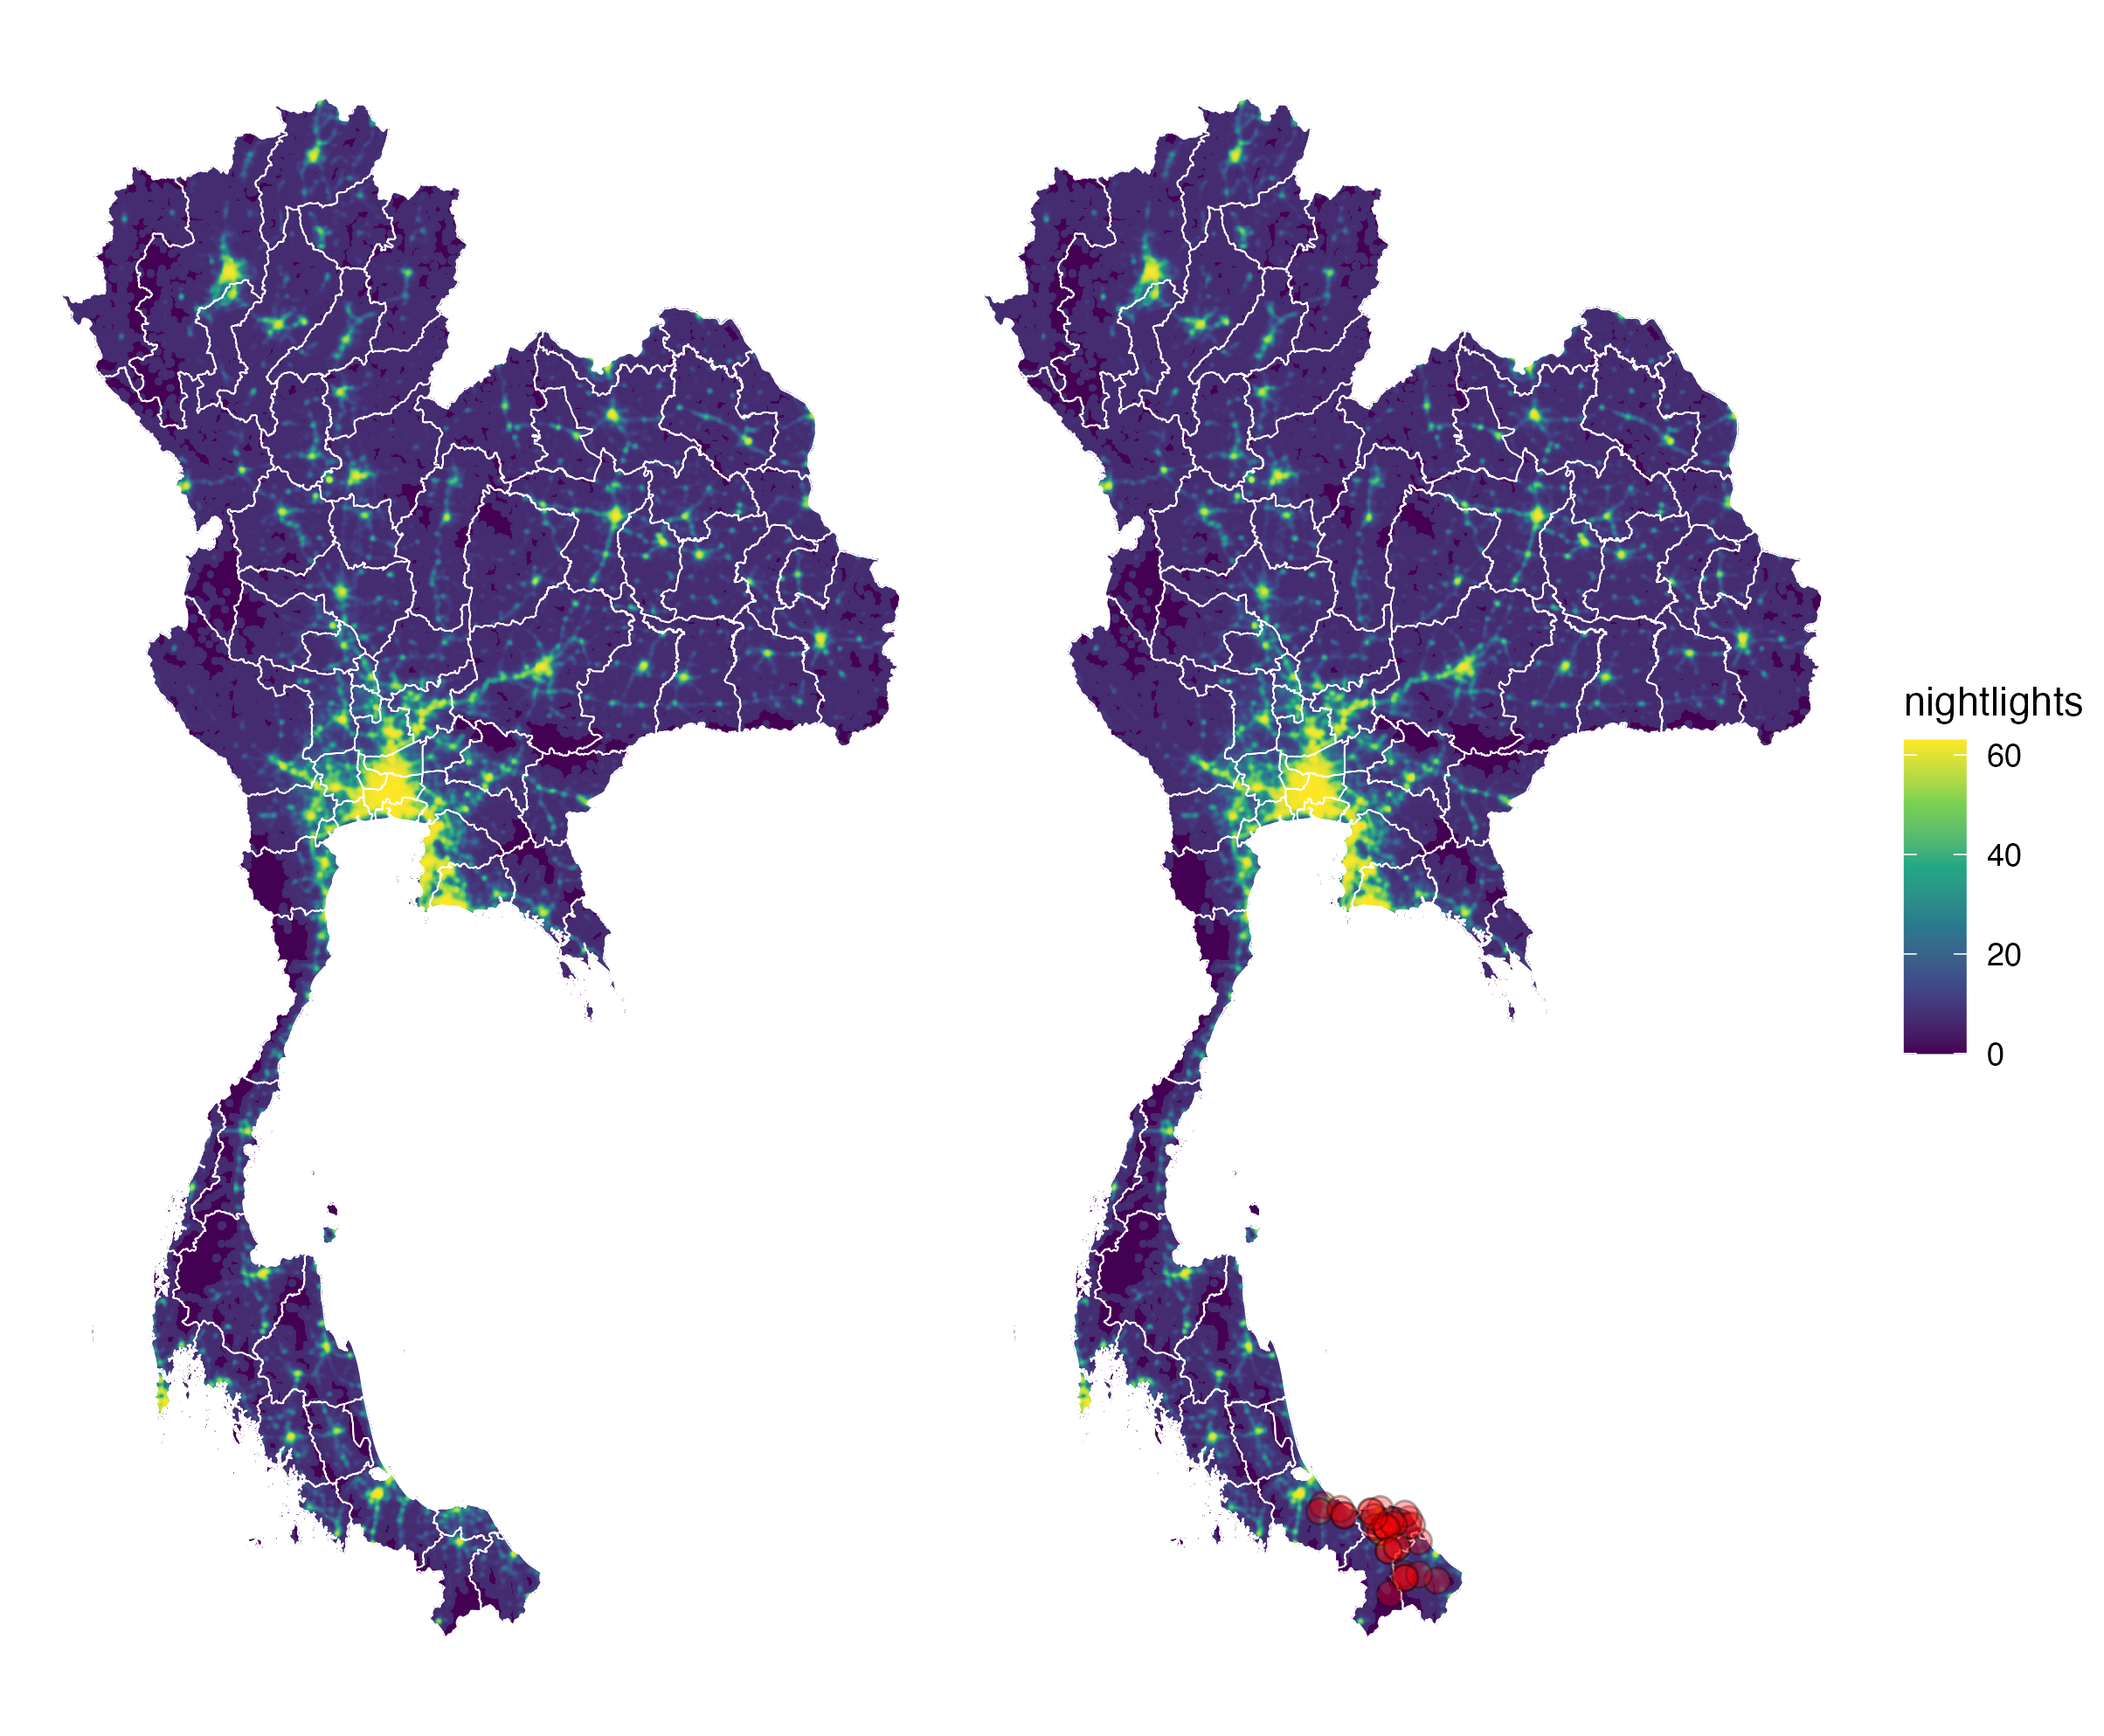
\includegraphics[width=\textwidth]{map_thailand_2020.png}
         \caption{2020}
         \label{fig:thailand2020}
     \end{subfigure}
    \begin{subfigure}[b]{0.45\textwidth}
         \centering
         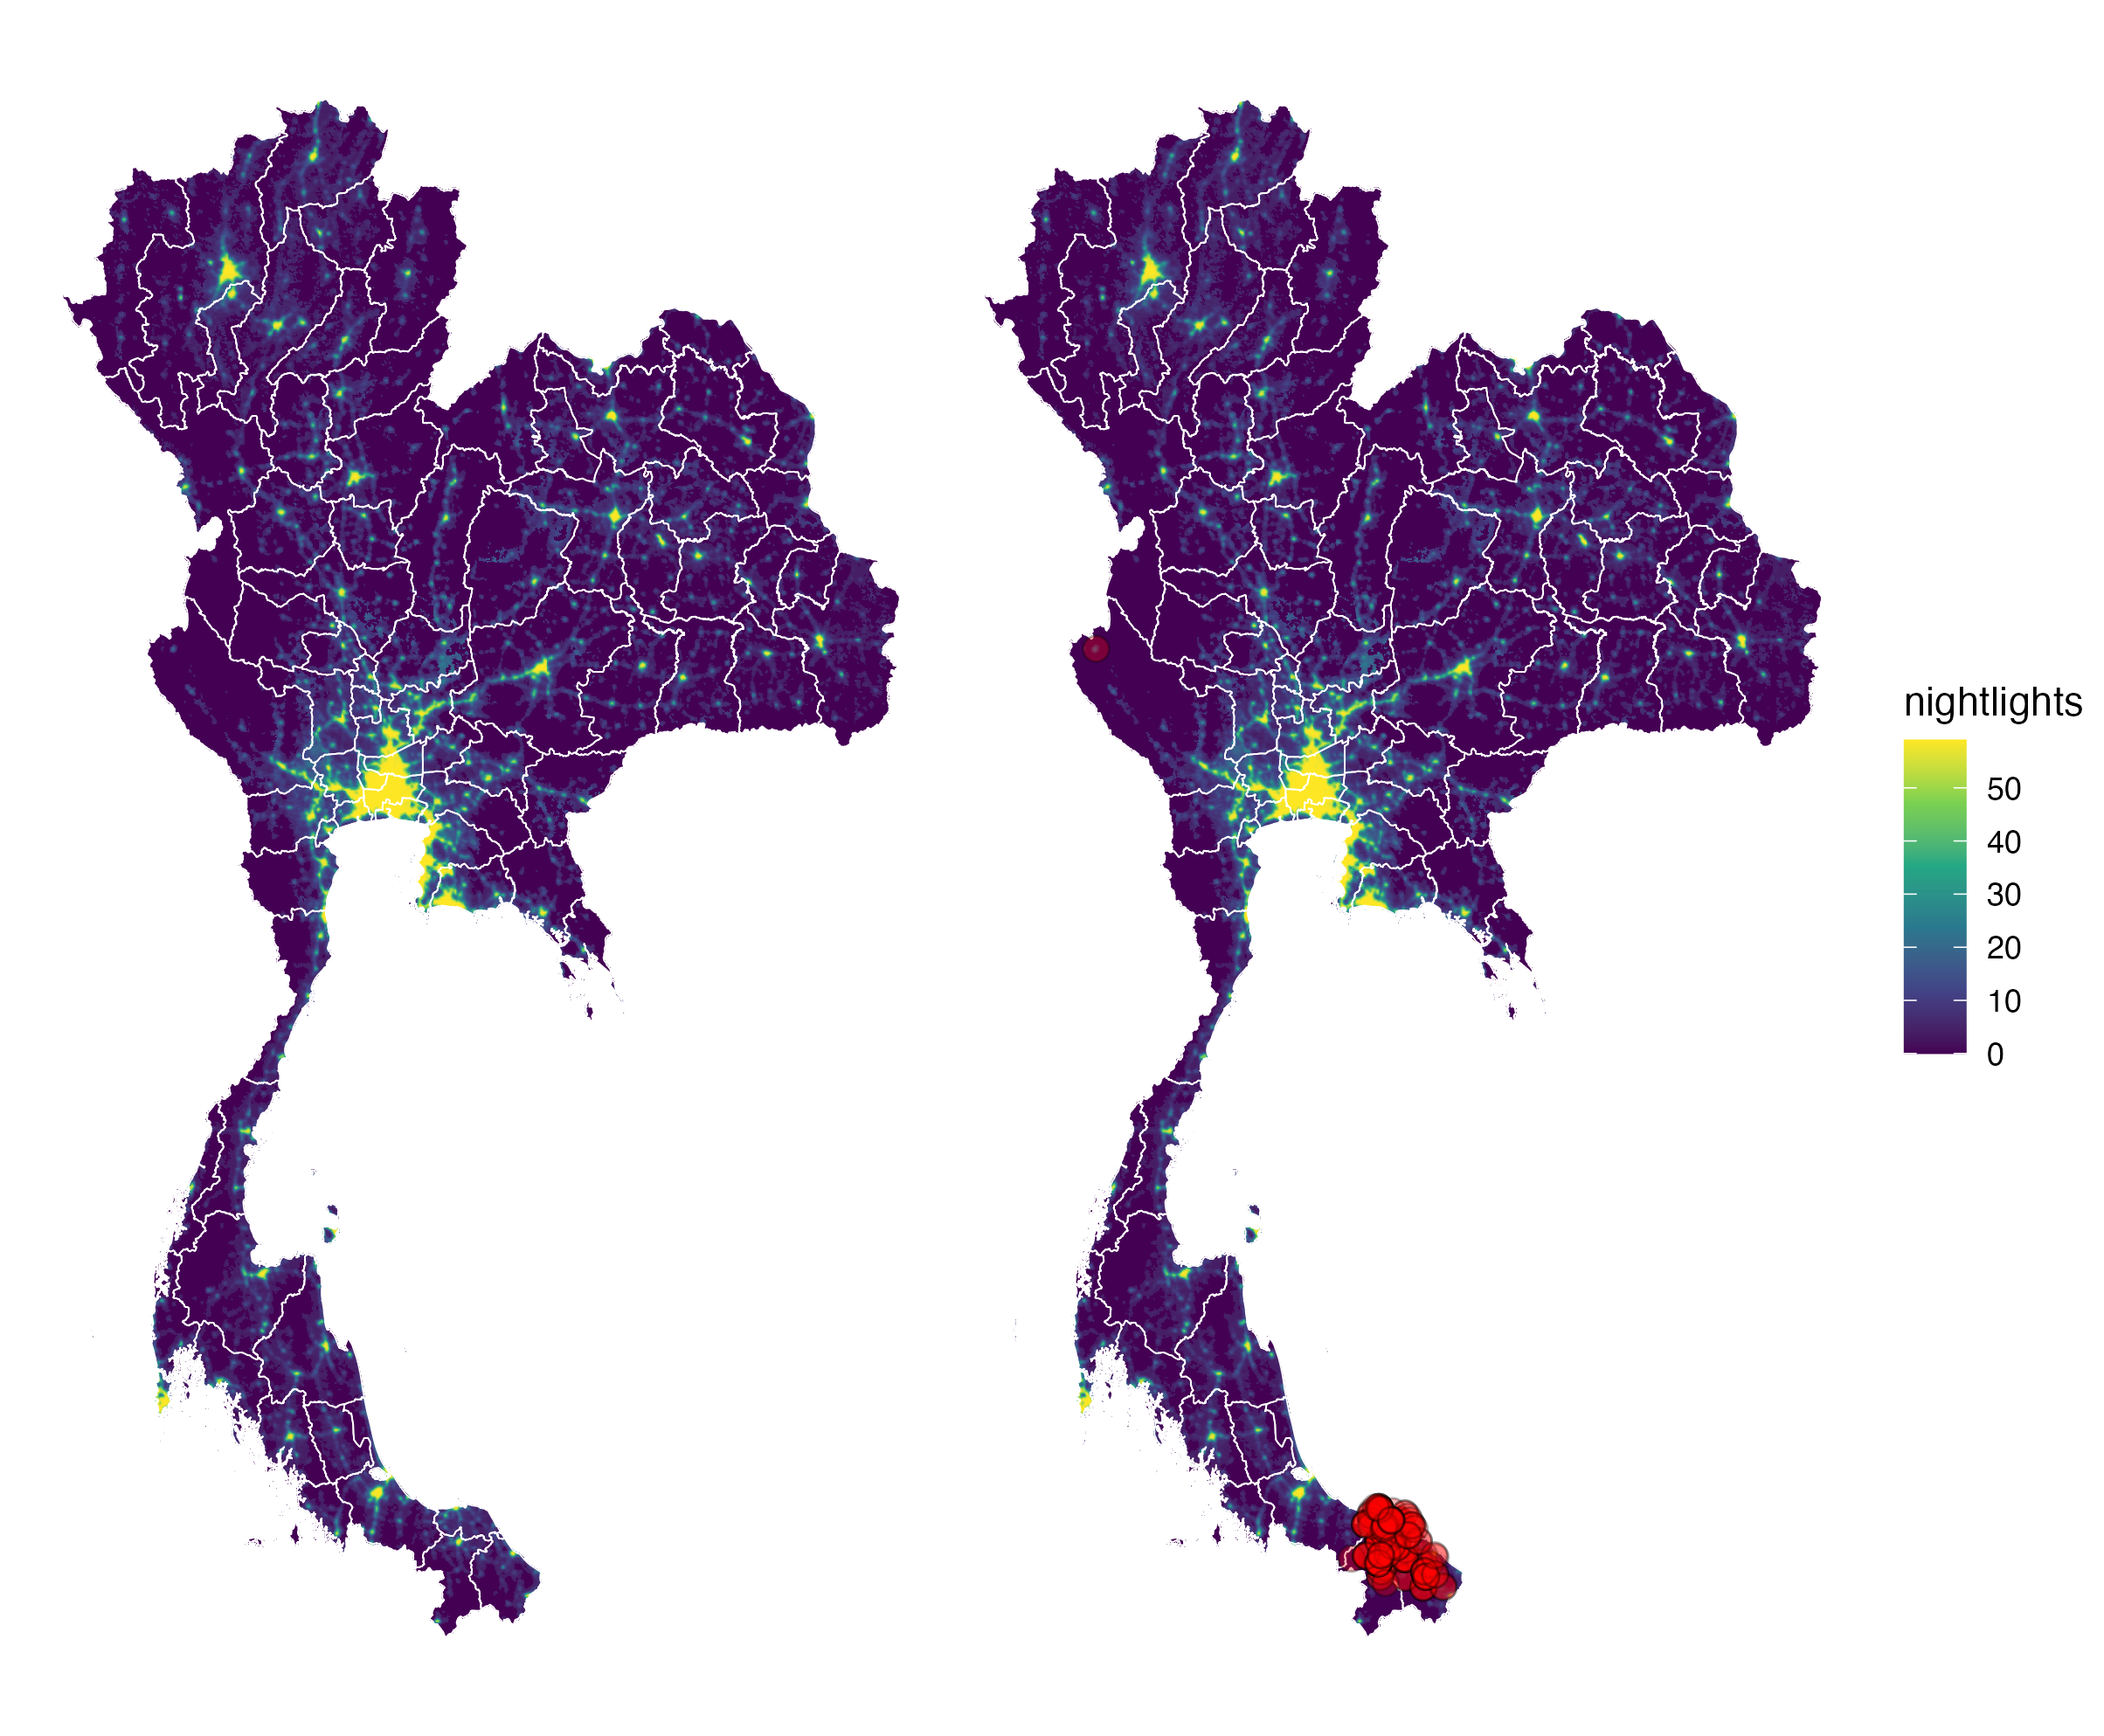
\includegraphics[width=\textwidth]{map_thailand_2010.png}
         \caption{2010}
         \label{fig:thailand2010}
    \end{subfigure}
    \caption{Conflict Events and Nightlight Intensity in Thailand. Year 2020 and 2010.}
    \label{fig:thailandmap}
\end{figure}

\section{Descriptive Statistics}
Next, Table \ref{tab:descrptive} represents the descriptive statistics of Thailand province-year panel data on the nightlight and conflict measure. There are 77 first-level provinces in Thailand, and the sample covers the period from 2010 to 2020. The variable \textit{nightlight mean} represents the average nightlight value in the given province in a particular year. \textit{Conflicts number} is the number of identified conflicts ongoing in a certain time and area, and \textit{conflicts events} is the total number of conflicts events occur in the province at a given year (the data unit of UCDP GED). A maximum of two types of conflict can occur in one province in one year, but 73 conflict events can occur in one province in a given year.

\begin{table}[htbp] \centering 
\begin{tabular}{@{\extracolsep{5pt}}lcccccc} 
\toprule
Statistic & \multicolumn{1}{c}{N} & \multicolumn{1}{c}{Mean} & \multicolumn{1}{c}{St. Dev.} & \multicolumn{1}{c}{Min} & \multicolumn{1}{c}{Median} & \multicolumn{1}{c}{Max} \\ 
\hline \\[-1.8ex] 
nightlight mean & 847 & 11.618 & 11.620 & 0.478 & 7.950 & 57.377 \\ 
conflicts number & 847 & 0.092 & 0.402 & 0 & 0 & 2 \\ 
conflicts events & 847 & 1.054 & 6.353 & 0 & 0 & 73 \\ 
\midrule
year & 11 &  &  & 2010 & & 2020 \\ 
province & 77 &  &  &  & &  \\ 
\bottomrule
\end{tabular} 
  \caption{Descriptive Statistics for Nightlight and Conflicts in Thailand} 
    \label{tab:descrptive} 
\end{table} 

\section{Discussion}
In conclusion, the preliminary analysis suggests promising avenues for future research into the relationship between night lights and conflicts. However, to conduct a causal relationship analysis, other factors affecting both nightlights and conflicts need to be taken into consideration. For instance, \textcite{Payo01102024} show the conflicts in the Southern Thailand have worsened the economy in such area, and the economy plays also an important role in the nightlight activities (\cite{gibson_which_2021}). Other factors such as ethnicity/cultural, government repression actions (both online and offline), and rural/urban areas can also have an impact. There may also be a time effect, considering that some conflicts last for several years or even decades. Therefore, more robust research methodologies need to be employed for casual reference studies, such as difference-in-difference analysis.

\section{Declaration of AI}
I use AI tools and internet sources, such as books and YouTube videos, to enhance my understanding of geographical information systems and respective coding implementation in R during this task. All codes and data are available at \href{https://github.com/YingYan77/thailand-conflict}{Github Page}. 

\printbibliography

\counterwithin{table}{section}
\appendix
\section{Appendix} 
\begin{table}[htbp]
    \centering
    \begin{tabular}{ccc}
\toprule
rank & country & conflicts\\
\midrule
1 & Afghanistan & 29248\\
2 & India & 4725\\
3 & Pakistan & 3963\\
4 & Philippines & 1714\\
5 & Myanmar (Burma) & 1152\\
6 & Thailand & 913\\
7 & Bangladesh & 135\\
8 & Indonesia & 78\\
9 & Tajikistan & 36\\
10 & Kyrgyzstan & 26\\
\bottomrule
\end{tabular}
    \caption{Ranking of aggregated conflicts events from 2010 to 2020 for Asian countries}
    \label{tab:my_label}
\end{table}

\end{document}
